\section{Experimental Study}
\label{sec:exp}

We introduce the experimental setup in \cref{sec:exp:setup} and test our \LLMQO comprehensively in the following facets: 
\ding{172} Compare the effectiveness of \LLMQO on three datasets with various baselines (\cref{sec:exp:compresult}) 
\ding{173} Explore the capability of model adaptation on unseen templates (\cref{sec:exp:generalization})
\ding{174} Investigate the adaptability of \QDPO with respect to new preference data (\cref{sec:exp:preference adaption})
\ding{175} Conduct an ablation study on prompt design of \QueryInstruct and LLM backbones (\cref{sec:exp:ablation}) 
\ding{176} Investigate the sensitivity of \LLMQO regarding parameter configurations (\cref{sec:exp:parameteranalysis}) 
\ding{177} Analyze the invalid plans generated by \LLMQO (\cref{sec:exp:validity_analysis})
\ding{178} Conduct case studies on visualized plans (\cref{sec:exp:case_study}) 
\ding{179} Evaluate the plan generation time of \LLMQO (\cref{sec:exp:time}). 

\subsection{Experimental Setup}
\label{sec:exp:setup}
\stitle{Datasets.}
We use 2 relational datasets, \imdb and \tpcds. 
For \imdb \cite{DBLP:conf/job/Leis18}, we use 6 relations, including \textsf{title}, \textsf{cast\_info}, \textsf{movie\_info}, \textsf{movie\_companies}, \textsf{movie\_info\_idx}, \textsf{movie\_keyword}.
There are 18 attributes and 6 PK/FK join conditions in total. 
\tpcds benchmark \cite{DBLP:conf/tpcds/Poess02} contains 24 relations and includes both PK/FK joins and non-PK/FK many-to-many joins. We use a scale factor of 5.
%We use three relational datasets: IMDB, JOB-light, and DSB to evaluate the performance of our \LLMQO.

\stitle{Queries.}
We use three query sets where two query sets are for \IMDB and one is for \tpcds. For the dataset \imdb, we construct a large query workload including query types supported by existing baselines, i.e., PK/FK join queries without selection conditions on the join attributes. We generate query sets with the number of PF/FK joins, $t$, varying from $0$ to $|T| -1$, where $|T|$ is the number of involved relations. 
To generate a query with $t (t > 0)$ joins, firstly a starting relation is uniformly sampled, and then the query is constructed by traversing from the starting relation over the join graph in $t$ steps. 
Here, for each relation in the sampled join query, additional selection predicates are drawn independently. 
For each $t$, $1,000$ queries are generated for \imdb.
Additionally, we generate a large query set of \job. \job, derived from the Join Order Benchmark (JOB)~\cite{DBLP:journals/pvldb/LeisGMBK015}, comprises 70 hand-written join queries that are suitable for serving as query templates, as each query is different from others in the involved set of relations and/or the selection predicates. 
We generate 100 queries for each template by uniformly drawing the literals of the predicates in their corresponding range.  
\dsb~\cite{ding2021dsb}, built upon the \tpcds benchmark, provides 15 SPJ query templates to assess the performance of DBMS, which enlarges the distinction of queries by introducing various join and selection patterns.  
We use templates tpl018, tpl019, tpl027, tpl040, tpl050, tpl084, tpl091, tpl099, tpl101, and tpl102, and generate 100 queries for each template following the same manner as \job. 
%Complicated templates whose execution are timeout in both \Postgres and \Oracle within 300 seconds are excluded.  
%timeout noun 
Complicated templates that exceed a time limit of 300 seconds in both \Postgres and \Oracle are excluded. 

\stitle{Baselines.}
We compare our \LLMQO with two traditional optimizers: the \Postgres (12.4), \Oracle (23.0) built-in optimizers, and two learned query optimizers: \bao and \hybrid.

\stitle{Evaluation Metrics.}
The generated plans of all the baselines are transformed into the format of \Postgres's physical plan, and then evaluated by the execution engine of \Postgres.
A \Postgres extension, pg\_hint\_plan~\cite{takaya2001nippon},
%\footnote{\url{https://pghintplan.osdn.jp/pg_hint_plan.html}} 
is used to transform the generated plans by \LLMQO into the execution plan of \Postgres. 
% Our evaluation primarily focuses on quantitative metrics that directly reflect the performance of \LLMQO from various perspectives. We outline these metrics as follows:
% 1) query plan execution time: This metric serves as the "gold standard" for query optimizers, providing a direct measure of the efficiency of the generated query plans.
We use the execution time of the generated plans as our evaluation metric. 

\stitle{Implementation \& Parameter Setting.} 
The learning framework of \LLMQO is built on PyTorch~\cite{pytorch} with Unsloth~\cite{unsloth}
%\footnote{\url{https://github.com/unslothai/unsloth}}
, a LoRA-based fine-tuning framework, which is designed for fast and resource-efficient training of LLMs. We use LLaMa-3-8B~\cite{DBLP:journals/corr/abs-2407-21783} as the default LLM backbone. 
%In the ablation studies, we additionally utilize LLaMa-2-7B\footnote{\url{https://huggingface.co/unsloth/llama-2-7b-bnb-4bit}}, CodeLLaMa-2-7B\footnote{\url{https://huggingface.co/unsloth/codellama-7b-bnb-4bit}}, and Mistral-7B\footnote{\url{https://huggingface.co/unsloth/mistral-7b-v0.3-bnb-4bit}}.
%
The models are trained with the AdamW~\cite{DBLP:conf/iclr/LoshchilovH19} optimizer, utilizing a learning rate of $2 \times 10^{-4}$ and $5 \times 10^{-6}$, for \QIT and \QDPO, respectively. For all datasets, the training steps $T$ are set to 600 and 200 for \QIT and \QDPO, respectively. The training batch size is set as 8.
By default, $r_0$ in Algorithm~\ref{alg:pdg}, $\beta$ in Eq.~\eqref{eq:u_function} are set to 0.95 and 0.1, respectively, and data is split by 80\% for training and 20\% for testing. 
Model training and inference are performed on a Tesla A100 GPU with 80GB memory. 
%
The experiments for query evaluation are conducted on \Postgres 12.4, 
whose execution engine is deployed on a Linux server with 96 CPUs and 512GB RAM. We set up \Postgres with 128MB shared buffers and 2GB working memory. 
For each query, we clean up the shared buffer of \Postgres and the Linux kernel buffer to fulfill a cold start. 

\subsection{Overall Effectiveness}
\label{sec:exp:compresult}
In this section, we compare \LLMQO with two traditional optimizers \Postgres and \Oracle and two state-of-the-art learned optimizers \bao and \hybrid, across three query workloads. 
For learned optimizers, training and test queries are randomly split by $8:2$. 
Table~\ref{tab:main_results} reports the mean, median, 75th, 95th, and 99th quantiles of the plan execution time. 
The mean and median provide an overview of the optimizers' performance, while other quartiles deliver the performance in long-tail cases. 
It is worth mentioning that all the plans generated by \LLMQO are valid. 
%Conclusion1:总体效果好;比traditional和learned都好
Table~\ref{tab:main_results} shows that \LLMQO 
outperforms both traditional and learned optimizers regarding most metrics across three workloads. 
We can observe that \LLMQO (\QIT) brings an remarkable performance gain over \Postgres across three query sets. 
In addition, \LLMQO (\QDPO) further reduces the average query execution time to 91.4\%, 94.4\%, and 31.3\% of \Postgres on \imdb, \job, and \dsb, respectively.
In general, the 95th and 99th quantiles are reduced by a large margin compared to \Postgres, showcasing that \LLMQO (\QDPO) effectively optimizes query execution time in long-tail scenarios.
In comparison to learned optimizers, \LLMQO outperforms them on average performance across three workloads as shown in Table~\ref{tab:main_results}, as training \LLMQO with \QueryInstruct enhances its ability to discover near optimal plans.
Specifically, \bao and \hybrid cannot surpass \LLMQO in long-tail cases of \imdb and \job, because they rely on coarse-grained hints and the limited plan exploration space makes it difficult for them to approach the optimal solution.
We observe that \bao achieves an impressive performance on \dsb, where \NestLoop is banned in about 76\% of the plans, indicating that certain hints are highly effective in specific workloads. 
It is worth noting that it is feasible to integrate the plan of learned optimizers, collaborating with traditional optimizers to further enhance the effectiveness and robustness of \LLMQO. 
%In future work, we will explore to integrate the behavior of learned optimizers such as \bao into \LLMQO, collaborating with traditional optimizers to further enhance its effectiveness and robustness.
In summary, 
our \LLMQO demonstrates the capability of generating valid and high-quality plans and outperforms both the traditional optimizers and learned optimizers in general cases. 


\begin{table*}[!t]
\centering
\small
    \caption{Execution time v.s. different optimizers across query sets. Best results are highlighted.}
\setlength\tabcolsep{2.5pt}
\begin{tabular}{lccccc|ccccc|ccccc}
\toprule
Execution time (sec)   & \multicolumn{5}{c}{{\imdb}}       & \multicolumn{5}{c}{\job} & \multicolumn{5}{c}{\dsb}   \\ \cmidrule(lr){1-1}\cmidrule(lr){2-6}\cmidrule(lr){7-11}\cmidrule(lr){12-16}
Method    & Mean  & Median & 75th  & 95th  & 99th   & Mean & Median & 75th & 95th & 99th  & Mean & Median & 75th & 95th & 99th \\ \midrule
\textbf{\Postgres} & 27.88 & 8.06 & 14.52 & 119.20 & 429.36 & 9.94 & 3.01 & 7.08 & 39.34 & 123.17 & 9.64 & 3.45 & 5.03 & 43.91 & 136.27\\ 
\textbf{\Oracle}     & 26.49 & 8.99 & \cellcolor{LightCyan}{13.60} & 108.47 & 389.78 & 10.11 & 3.03 & 10.00 & 38.96 & \cellcolor{LightCyan}{111.21} &5.45 &2.34 & 6.62 & 23.44 & 28.24 \\
\midrule
\bao & 28.10 & 8.05 & 15.36 & 121.71 & 435.53 & 10.07 & 2.71 & 7.14 & 39.46 & 123.60  & 3.09 & 2.48 & 3.99 & 11.74 & 12.21  \\ 
\hybrid & 27.55 & 7.73 & 13.79 & 120.04 & 427.01  & 9.97 & 3.02 & 7.06 & 39.15 & 124.97  & 9.14 & 2.89 & \cellcolor{LightCyan}{3.69} & 43.48 & 136.32  \\ \midrule
\LLMQO (\QIT)   
& 26.68 & 7.71 & 13.79 & 119.10 & 385.48
& 9.73 & 2.27 & 7.10 & 38.94 & 123.10 & 4.65 & 2.37 & 4.43 & 11.66 & 50.60 \\
\% of \textbf{\Postgres}   & 95.7\% & 95.7\% & 95.0\% & 99.9\% & 89.8\%  & 97.9\% & 75.4\% & 100.2\% & 99.0\% & 99.9\%  & 48.2\% & 68.6\% & 88.0\% & 26.6\% & 37.1\%\\ 




\LLMQO (\QDPO)   & \cellcolor{LightCyan}{25.48} & \cellcolor{LightCyan}{7.65} & 13.70 & \cellcolor{LightCyan}{107.86} & \cellcolor{LightCyan}{373.24}
& \cellcolor{LightCyan}{9.38} & \cellcolor{LightCyan}{2.27} & \cellcolor{LightCyan}{6.96} & \cellcolor{LightCyan}{38.86} & 115.94 & \cellcolor{LightCyan}{3.02} & \cellcolor{LightCyan}{2.33} & 3.74 & \cellcolor{LightCyan}{11.46} & \cellcolor{LightCyan}{11.72} \\
\% of \textbf{\Postgres}  & 91.4\% & 95.0\% & 94.4\% & 90.5\% & 86.9\% & 94.4\% & 75.4\% & 98.3\% & 98.8\% & 94.1\%  & 31.3\% & 67.6\% & 74.4\% & 26.1\% & 8.6\%\\ 






\bottomrule
\end{tabular}
%\vspace{10pt} 
\label{tab:main_results}
\end{table*}

\begin{table*}[!t]
\setlength\tabcolsep{2.5pt}
\centering
\small
\caption{Performance of out-of-distribution (OOD) templates. Best results are highlighted.}
\begin{tabular}{lccccc|ccccc|ccccc}
\toprule
Execution time (sec)   & \multicolumn{5}{c}{\imdb}       & \multicolumn{5}{c}{\job} & \multicolumn{5}{c}{\dsb}   \\ \cmidrule(lr){1-1}\cmidrule(lr){2-6}\cmidrule(lr){7-11}\cmidrule(lr){12-16}
Method    & Mean  & Median & 75th  & 95th & 99th   & Mean & Median & 75th & 95th & 99th  & Mean & Median & 75th & 95th & 99th \\ \midrule
\Postgres  & 86.59 & 36.73 & 82.64 & 416.37 & 483.57  & 31.09 & 9.11 & \cellcolor{LightCyan}{20.10} & 229.41 & 272.90 & 5.32 & 4.03 & 7.50 & 12.39 & 12.72\\ 
\Oracle        & 79.40 & 34.06 & 76.48 & \cellcolor{LightCyan}{374.90} & \cellcolor{LightCyan}{436.43}  & 30.59 & \cellcolor{LightCyan}{8.72} & 22.87 & {206.98} & {264.63} & 8.84 & \cellcolor{LightCyan}{2.37} & 19.31 & 24.98 & 29.76\\ \midrule
\bao & 86.68 & 36.65 & 82.85 & 417.81 & 484.65 & 31.25 & 9.21 & 20.60 & 229.36 & 273.29  
% & 4.41 & 2.50 & \cellcolor{LightCyan}{5.04} & 12.28 & 12.96  
& 4.41 & 2.50 & 5.49 & 12.08 & 13.02
\\ 
\hybrid & 86.27 & 36.86 & 83.05 & 411.35 & 479.15 & 31.28 & 9.20 & 20.05 & 230.78 & 273.83
& 4.88 & 3.75 & 6.74 & \cellcolor{LightCyan}{10.84} & \cellcolor{LightCyan}{11.17} \\
% hyqo model.eval off for DSB: & 4.69 & 3.50 & 6.47 & 10.33 & 11.29   
% \textbf{Bao}  & & & & &   & & & & &   & & & & & \\
\midrule
\LLMQO (\QIT)   & \cellcolor{LightCyan}{79.24} & \cellcolor{LightCyan}{33.12} & \cellcolor{LightCyan}{75.28} & 375.73 & 438.32 
% & \cellcolor{LightCyan}{30.20} & 8.99 & 24.06 & 208.56 & 265.05 
& \cellcolor{LightCyan}{29.93} & 8.74 & 22.40 & \cellcolor{LightCyan}{204.55} & \cellcolor{LightCyan}{263.36}
& \cellcolor{LightCyan}{4.40} & 2.39 & \cellcolor{LightCyan}{5.33} & 11.89 & 12.41\\ 
\% of \textbf{\Postgres}   & 91.5\% & 90.2\% & 91.1\% & 90.2\% & 90.6\%  %97.1\% & 98.6\% & 119.7\% & 90.9\% & 97.1\% 
& 96.3\% & 95.9\% & 111.5\% & 89.2\% & 96.5\%
& 82.8\% & 59.2\% & 71.1\% & 95.9\% & 97.5\%  \\
\% of \textbf{\Oracle}  & 99.8\% & 97.2\% & 98.4\% & 100.2\% & 100.4\% 
% & 98.7\% & 103.0\% & 105.2\% & 100.8\% & 100.2\% 
& 97.8\% & 100.2\% & 98.0\% & 98.8\% & 99.5\%
& 49.8\% & 100.9\% & 27.6\% & 47.6\% & 41.7\%\\ 
\bottomrule
\end{tabular}
\vspace{-1ex}
\label{tab:ood_performance}
\end{table*}

\subsection{Generalization to OOD Queries}
\label{sec:exp:generalization}
% To study the generalization capability of LLMs on out-of-domain (OOD) templates, we evaluate the performance of \LLMQO on three OOD test sets. 
%learned optimizers 其实很难在OOD的场景下有较好的表现、LLM
%Motivated by the promising performance of \LLMQO in general cases, we further explore its ability for OOD generalization. 
We study the performance of \LLMQO in OOD scenarios, where test queries are in completely different query templates from those of the training queries, to verify the generalizability of \LLMQO.
% in a difficult scenario, where the test queries are out-of-distribution. 
% The architecture of fine-tuned LLMs enables them to understand complex patterns and relationships in language, resulting in improvements for OOD generalization.
% In this section, we consider a challenging partitioning of the training and testing datasets, in which we evaluate model performance using out-of-domain (OOD) templates. 
% we ensure that all queries corresponding to the same base query are exclusively assigned to either the training set or the test set.
% In this setting, query templates in the train
% and test sets are completely disjoint, allowing us
% to evaluate our method for unseen queries.
For \imdb and \job, we use the most challenging queries, queries with 5 tables as the test queries, and train \LLMQO using queries with $2\sim 4$ tables.
%select q5, as well as q66 and q70 for testing, respectively.  
%These test queries are of 5 joins and considered difficult across all the templates.
For \dsb, we use three query templates with 5, 6 and 12 joins as test queries, while the remaining templates are used as training queries. 
Table~\ref{tab:ood_performance} shows the plan execution time of \LLMQO (\QIT) compared to baseline optimizers on the three query sets. 
In general, \LLMQO consistently outperforms \Postgres on OOD queries by a statistically large margin, 
indicating that \LLMQO can efficiently explore the plan space to obtain better plans.
In addition, \LLMQO achieves competitive performance compared with the state-of-the-art learned optimizers, \bao and \hybrid.
The coarse-grained hint-based optimization of \bao achieves a low query execution time on \dsb 
by average, however, all the listed quantiles are inferior to those of \LLMQO. Moreover, we observe that the 95th and 99th quantiles of \hybrid are lower than those of \LLMQO.
In addition, we try to further fine-tune LLM in \QDPO stage by using queries with OOD templates and test new queries with these templates, however, the corresponding \LLMQO (\QDPO) suffers from generating a large fraction of invalid plans. 
This phenomenon indicates that a
negative effect occurs when using fully unseen query templates to fine-tune LLMs in \QDPO stage, which suggests that the robustness of LLMs should be further improved by smoothing the transition from \QIT to \QDPO and leveraging more abundant training data.


\subsection{Adapting to New Preferences}
\label{sec:exp:preference adaption}
To study the adaptability of \LLMQO to possibly new plan preferences through \QDPO stage, we add \db (v12.1) built-in optimizer into Algorithm~\ref{alg:pdg} as an additional source of training plans and construct a new preference training dataset $\mathbb{D}_\mathrm{dpo}^+$ by the optimizers of \Postgres, \Oracle, and  \db  for \dsb. 
Afterwards, we conduct \QDPO training with $\mathbb{D}_\mathrm{dpo}^+$ on \LLMQO (\QIT) and obtain \LLMQO (\QDPO)$^{+}$, in contrast to \LLMQO (\QDPO). 
Fig.~\ref{fig:exp:preference_adaption} compares the average query execution time per template for  the baselines, and the three \LLMQO variants on 200 test queries from \dsb.
%
In general, we observe that \LLMQO (\QDPO)$^{+}$ achieves the overall best performance across all {\LLMQO}s.
In comparison to \LLMQO (\QIT), \LLMQO (\QDPO) and \LLMQO (\QDPO)$^{+}$ significantly reduce
the execution time on templates tpl018, tpl019, and tpl040, and achieve comparable performance on the remaining templates. 
%
Fig~\ref{fig:exp:preference_adaption} illustrates that \db outperforms both \Postgres and \Oracle on tpl027. Therefore, the plans generated by \db will be regarded as the preferred plans in $\mathbb{D}_\mathrm{dpo}^+$. \LLMQO (\QDPO)$^{+}$ exhibits performance improvement on tpl027, exceeding that of \LLMQO (\QIT) and \LLMQO (\QDPO), which supports our envision that LLMs can adapt to new preferences and generate more efficient plans in \QDPO stage.
%
However, we find that \LLMQO (\QDPO)$^{+}$ cannot improve  performance on tpl091, although \db performs better than \Postgres and \Oracle.
This is because the training plans in \QIT stage are from \Oracle for all the queries with tpl091. The behavior of \LLMQO (\QIT) is dominated by \Oracle's preference, and is relatively hard to adapt to more preferences in \QDPO stage. 

\begin{figure}
  \centering
 \includegraphics[width=0.45\textwidth]{figures/preference_adaption/dsb_time/dsb-figure0.pdf}
  \caption{Preference Adaption on \dsb}
  \vspace{-2ex}
\label{fig:exp:preference_adaption}
\end{figure}
\subsection{Ablation Studies}
\label{sec:exp:ablation}
In this section, we conduct ablation studies on different components of \LLMQO, from the perspectives of input features, output format, and LLM backbone to justify the design rationale behind \LLMQO. Table~\ref{tab:ablation} lists the performance of these \LLMQO variants on \dsb.

\subsubsection{Input Features}
As introduced in \cref{sec:method:query_instruct:prepare}, 
%the input features of \LLMQO consist of an SQL query, the statistics of the schema associated with the SQL query, and an input-output pair as the one-shot demonstration for controlling the format. 
the auxiliary statistical information of the database schema and the planning demonstration are important features of \QueryInstruct.  
We remove the statistical information and the one-shot demonstration from the prompt to test their impact on \QueryInstruct respectively. 
As shown in the first part of~Table~\ref{tab:ablation}, compared with the intact version \LLMQO, removing the database statistics feature results in substantial performance degradation.
This result indicates the importance of incorporating data distributions of tables into the plan generation task, which is quite similar to the importance of catalogs to traditional query optimizers. 
In addition, we notice that the withdrawal of the demonstration significantly hurts the performance
on all evaluation metrics. 
This is because the demonstration provides a positive reference for the input query and helps regulate the plan space, and this mechanism is beneficial for plan generation using \LLMQO.
These results further implicitly verify that \LLMQO can understand both the statistics and the demonstration. 

\subsubsection{Output Format}
In \QueryInstruct, we adopt the planning path together with a bracket sequence  as the output format. 
To assess the effectiveness of the planning path, we remove it by only using the bracket answer (Fig.~\ref{fig:example:bracket_sequence})  as an ablation. In the second part of Table~\ref{tab:ablation}, we observe that
the \QIT model yields competitive results, but the performance of the \QDPO model is worse than that of its full version counterpart. 
% This indicates that utilizing this output format during the DPO stage leads to noticeably poorer performance compared to \LLMQO (\QDPO), which
This finding indicates that the planning path enables the model to differentiate between plain and good plans at a fine-grained level during \QDPO stage, therefore improving the model performance.

\comment{
% \noindent\textbf{Direct Plan: Directly output the plan.
% }

% \noindent\textbf{Hint-style Plan: The plan can be deconstructed into two distinct sequences: the output join algorithm and the join order.
% }
}
\subsubsection{LLM Backbone}
To explore the capabilities of different LLM backbones for the query optimization task, we adopt Mistral-7B~\cite{jiang2023mistral}, CodeLLaMA-7B~\cite{roziere2023code}, and LLaMA2-7B~\cite{touvron2023llama},  respectively to replace the default LLM, LLaMA3-8B, in \LLMQO. 
% In Table~\ref{tab:ablation}, they are denoted as ``CodeLLaMA-7B'', ``LLaMA2-7B'', and ``Mistral-7B''.
As shown in Table~\ref{tab:ablation}, our proposed framework brings improvements across various LLM backbones regarding plan execution time during \QIT and \QDPO stages, affirming its general applicability and superiority.
%Comparison of LlaMa2 and LlaMa3
In addition, the performance of CodeLLaMA-7B and LLaMA2-7B are comparable to that of \LLMQO after \QDPO stage, better than that of Mistral-7B. This phenomenon suggests that LLaMA models may well-suited for the query optimization task. 
%
It is noteworthy that Mistral-7B after \QDPO stage suffers from the risk of invalid generation.
We observe that the model outputs a large amount of redundant content before performing the plan generation, which is frequently observed in generative models~\cite{DBLP:conf/iclr/HoltzmanBDFC20}.



\begin{table}
\centering
\caption{Ablation studies of \LLMQO on \dsb}
\centering
% \small
\begin{adjustbox}{width=0.48\textwidth}
%\setlength{\tabcolsep}{6pt} % Reduce the space between columns
\renewcommand{\arraystretch}{0.8} % Adjust the value as needed, 1.5 is 50% larger
\label{tab:ablation}
\begin{tabular}{@{}l|cccccc@{}}
\toprule
Model Variants     & Mean  & Median & 75th  & 95th & 99th  &invalid\\ 
\midrule
\textbf{\Postgres}     & 9.64 & 3.45 & 5.03 & 43.91 & 136.27 &-
% \textbf{Oracle}     &5.45 &2.34 & 6.62 & 23.44 & 28.24 \\
\\ \midrule
Input Features      &  &  &  &  &\\
\quad- \textit{w/o} statistics (\QIT) & 6.28 & 2.41 & 4.25 & 11.74 & 61.91 &-\\
\quad- \textit{w/o} statistics (\QDPO) & 4.58 & 2.39 & 4.24 & 11.63 & 50.03 &-\\
\quad- \textit{w/o} demo (\QIT)  & 6.16 & 2.61 & 4.47 & 32.96 & 62.15 &- \\
\quad- \textit{w/o} demo (\QDPO)  & 5.09 & 2.39 & 4.17 & 11.59 & 37.37 &1  \\
\midrule
Plan Output Format      &  &  &  & &  \\
\quad- \textit{w/o} planning path (\QIT)    & 5.03 & 2.49 & 4.35 & 11.90 & 53.19 &-\\ 
\quad- \textit{w/o} planning path (\QDPO) & 4.24 & 2.54 & 4.24 & 11.60 & 47.59 &-
% \quad- Hint-style Plan    &  &  &  & 
\\ \midrule
Backbones      &  &  &  & & \\
\quad- CodeLLaMA-7B (\QIT)     & 6.40 & 2.76 & 4.48 & 34.50 & 61.86 &- \\
\quad- CodeLLaMA-7B (\QDPO)      & 3.12 & 2.39 & 3.81 & 11.61 & 11.87 &- \\
\quad- LLaMA2-7B (\QIT)    & 5.15 & 2.50 & 4.24 & 11.61 & 51.78 &-\\
\quad- LLaMA2-7B (\QDPO)  & 3.07 & 2.37 & 3.70 & 11.53 & 11.69 &- \\
\quad- Mistral-7B (\QIT)  & 6.38 & 2.81 & 4.46 & 34.42 & 62.17  &- \\
\quad- Mistral-7B (\QDPO)    & 5.71 & 2.61 & 4.48 & 18.92 & 59.69 &34\\  \midrule
\textbf{Full version}     &  &  &  &  &\\
\quad- \LLMQO (\QIT)     & \textbf{4.65} & \textbf{2.37} & \textbf{4.43} & \textbf{11.60}  &\textbf{50.60} &-\\ 
\quad-  \LLMQO (\QDPO)     & \textbf{3.02} & \textbf{2.33} & \textbf{3.74} & \textbf{11.46} & \textbf{11.72} &-
\\
% \quad Mistral w/o Pre-training        & xx (60.4\%) & xx (52.3\%) & xx (20.1\%) & xx (15.9\%) \\ 
\bottomrule

\end{tabular}
\end{adjustbox}
\renewcommand{\arraystretch}{1.0}
\vspace{-2.5ex}
\end{table}



% \vspace*{-0.1cm}
\begin{figure*}[t]
\begin{center}
\begin{tabular}[t]{c}
% \hspace{-0.5cm}
   \subfigure[Varying the scale of \QIT training data]{
   \label{fig:params:scale_sft}
     \includegraphics[width=0.50\columnwidth]{figures/parameter_analysis/SFT.pdf} 
    }
       % \hspace{-0.3cm}
    \subfigure[Varying the scale of \QDPO training data]{
      \label{fig:params:scale_dpo}
      \includegraphics[width=0.50\columnwidth]{figures/parameter_analysis/DPO.pdf} 
    }
    \subfigure[Varying the threshold $r_{0}$ ]{
      \label{fig:params:r_0}
      \includegraphics[width=0.50\columnwidth]{figures/parameter_analysis/THRE.pdf}
      }
    \subfigure[Varying the coefficient $\beta$ ]{
      \label{fig:params:beta}
      \includegraphics[width=0.50\columnwidth]{figures/parameter_analysis/BETA.pdf} 
    }
\end{tabular}
\end{center}
% \vspace*{-0.2cm}
\caption{The impact of training data scale,  $r_{0}$, and $\beta$ on \dsb}
\label{fig:parameter}
\end{figure*}


\subsection{Parameter Analysis}
\label{sec:exp:parameteranalysis}
We study the parameter sensitivity of \LLMQO w.r.t. three key hyper-parameters: (1) the scale of the training data, (2) the threshold $r_0$ in Algorithm~\ref{alg:pdg} and (3) the coefficient $\beta$ for controlling the divergence of $\pi_\mathrm{dpo}$ from $\pi_\mathrm{sft}$. 
In general, Fig.~\ref{fig:parameter} shows the plan execution time on \dsb for different model variants, where the points `$\times$' and `$\bullet$' denote the mean and 95\% quantiles, respectively. 
%\tjadd{ do we need to explain the lower and upper bound of box?}
%
\subsubsection{Impact of training data scale} 
Fig.~\ref{fig:params:scale_sft}-\ref{fig:params:scale_dpo} show how the scale of training data affects the performance of \LLMQO models on \dsb, in the first and second fine-tuning stages respectively.
LLMs have been observed to possess high data efficiency on text-to-text NLP tasks, achieving competitive performance with a small proportion (e.g., 0.5\%) of full training data~\cite{DBLP:journals/corr/abs-2305-09246}. We study this in the query planning task. 
Specifically, we evaluate the performance of LLaMA3-8B when training on \dsb with different sizes. In the two-stage training, we randomly sample 25\%, 50\%, 75\%, and 100\% of the data from $\mathbb{D}_\mathrm{sft}$ and $\mathbb{D}_\mathrm{dpo}$, respectively. 
%SFT model
In Fig.~\ref{fig:params:scale_sft}, we find a declining trend in execution time as the volume of training data increases for the \QIT models.
Unlike previous observations\cite{DBLP:journals/corr/abs-2305-09246}, the model does not reach its peak performance until using full training data. The reason may be that the structured output of the plan generation task is more challenging for generative LLMs compared to other text-based tasks.
%DPO model
In Fig.~\ref{fig:params:scale_dpo}, we also observe a moderate improvement as the scale of training data increases. 
The data scale $=0$ indicates that the model bypasses \QDPO stage.
We find that the model without DPO fine-tuning cannot achieve results comparable to those achieved by
\LLMQO (\QDPO) models. It is worth noting that the \LLMQO (\QDPO) model can achieve high performance even though the data ratio is as small as 25\%. These findings confirm that the effectiveness of \QDPO stage in \LLMQO when training data is limited.

\comment{
\begin{table}[!t]
\centering
\caption{Performance comparison on the \dsb
dataset with different training data scale in the SFT stage.}
%\setlength\tabcolsep{2.5pt}
\begin{tabular}{lccccc}
\toprule
Execution time (sec)   & \multicolumn{4}{c}{\textcolor{blue}{DSB}}  \\ \cmidrule(lr){1-1}\cmidrule(lr){2-6}
Data size   & Mean  & Median & 75th  & 95th & 99th \\ \hline \hline
25\% & 6.49 & 2.94 & 4.69 & 35.00 & 62.84 \\ \hline
50\% & 5.97 & 2.85 & 4.61 & 18.81 & 62.15 \\ \hline
75\% 
& 5.74 & 2.36 & 4.38 & 11.78 & 59.97
\\ \hline
% 100\% & \textbf{4.65} & \textbf{2.37} & \textbf{4.43} & \textbf{11.66} & 
100\% & 4.65 & 2.37 &4.43 & 11.66 & 50.60  \\
\bottomrule
\end{tabular}
%\vspace{10pt}

\label{exp:tab:data scale sft}
\end{table}
}

%Figure
\comment{
\begin{figure}
  \centering
 \includegraphics[width=0.45\textwidth]{figures/parameter/parameter_scale_up_sft.pdf}
  \caption{Performance comparison on the \dsb dataset with different training data scale in the SFT stage.}
\label{fig:experiment:scale_up_sft}
\end{figure}
}

\subsubsection{Impact of the threshold $r_0$} 
Recall that \LLMQO introduces the threshold $r_0 \in (0, 1)$ that influences the preference plan generation in \cref{sec:queryinstruct:PDG}.
% Fig.~\ref{fig:params:r_0} shows how the threshold $r_0$ affects the model performance on \dsb.
In Fig.~\ref{fig:params:r_0}, we present the plan execution time for different values of $r_0$, specifically in the range of $\{0.6, 0.7, \cdots, 1.0\}$. 
Algorithm~\ref{alg:pdg} shows that larger values of $r_0$ will increase the volume of preference data. However, setting $r_0$ too large may lead to $\bm{y}_w$ and $\bm{y}_l$ sharing similar quality, potentially impeding the optimization process and model convergence.
%
When $r_0$ is set between 0.60 and 0.80, the  performance of the model is significantly better than that of 0.90 and 1.00. 
The remarkable performance degradation can be attributed to the fact that in the settings of 0.90 and 1.00, the training data faces a high risk of uncertainty, where the statistical performance dominance is insignificant. 
The best performance is achieved at 0.80 as it increases the size of preference data without compromising its quality.
%
Therefore, establishing a balanced threshold is essential for optimizing model training and enhancing overall performance.

\begin{table}[t]
	\centering
\caption{The number of invalid cases across three query sets under different \QueryInstruct settings in OOD scenarios}	
	%\footnotesize
        \small 
			\begin{tabular}{l|l|c c c c}
			\toprule
                \multirow{1}{*} {Datasets}  &{\QueryInstruct Variants} 
                
			& \textbf{E1} & \textbf{E2} & \textbf{E3} & {Total} \\ \midrule     
      		\multirow{2}{*}
%50 samples in total
            {\centering \imdb}	&(a) \textit{w/o} demo          
            &3  &0   &0  &3
            % &1  &0   &13  &14
            % &0 & 0 & 25 & 25 
            \\
       	& (b) \textit{w/o} planning path            &0 &0  &0  &0  \\

            	& (c) \textit{w/o} both           %&4 &0  &0  &4 
                 % &1 &0  &2  &3
                &16 &0  &6  &22
                % &2 & 0 & 32 & 34
                \\
                     	& (d) \textbf{Full version}            &0 &0  &0  &0  

       \\ \midrule

%40 samples in total
		\multirow{2}{*}{\centering  \job} &(e) \textit{w/o} demo         
        &10  &0 &0 &10  
         % &20 &0  &0  &20
         \\
  
		&(f) \textit{w/o} planning path     &0  &0   &1  &1
\\
  
            	& (g) \textit{w/o} both          %&1 &0  &2  &3  
               &16 & 0 & 5 & 21 
                
                \\
                     	& (h) \textbf{Full version}            &0 &0  &0  &0  
                      
  \\ \midrule
%60 samples in total
  		\multirow{2}{*}{\centering \dsb} &(i) \textit{w/o} demo      
        % &14 &3    &3   &20 
        &16 &4    &3   &23
        
        \\
  
		&(j) \textit{w/o} planning path   
        % &1 &0  &3 &4 
                &1 & 0 & 14 & 15
        
        \\
  
            	& (k) \textit{w/o} both          %&10 &1  &11 &22    
                &14 & 3 & 12 & 29 
                \\
                     	& (l) \textbf{Full version}            &0 &0  &1  &1  
  
  \\ 
     \bottomrule
		
		\end{tabular}	

	\label{exp:tab:invalid analysis}
        \vspace{-1.0ex}
\end{table}

\subsubsection{Impact of the hyper-parameter $\beta$} 
As described in Algorithm \ref{alg:dpo}, \QDPO stage involves a hyper-parameter $\beta$, which controls the divergence of $\pi_\mathrm{dpo}$ from $\pi_\mathrm{sft}$.
% The added constraint prevents the model from deviating too far from the distribution on which the reward model is accurate and maintains the generation diversity. 
In Fig.~\ref{fig:params:beta}, we vary $\beta$ in its empirical range, \{0.01, 0.05, 0.1, 0.3, 0.5\}, and show the performance of \LLMQO (\QDPO).
Notably, we observe that a large $\beta$, which is correlated with greater knowledge retention, leads to a significant performance drop, indicating its pivotal role in controlling the extent of knowledge  preservation in \QDPO models. 
Conversely, setting $\beta$ to 0.01 substantially weakens the effort in the first-stage training, resulting in a decline in model performance.
The superior performance is achieved with moderate $\beta$ values in 
$\{0.05, 0.1, 0.3\}$.

\subsection{Invalid Plan Analysis}
\label{sec:exp:validity_analysis}
In our experiments, we observe that in OOD scenarios, the plans generated by \LLMQO suffer from different degrees of invalidation across the three query sets.
Therefore, we conduct an in-depth analysis on the effectiveness of the two features in  \QueryInstruct, the planning demonstration and the planning path, in OOD scenarios. 
% We remove the one-shot demonstration and planning path from the prompt to test their impact on \QueryInstruct, respectively. 
%The results are summarized
%in Table~\ref{exp:tab:invalid analysis}.
Table~\ref{exp:tab:invalid analysis} lists the number of invalid cases across the three query sets. 
Specifically, we categorize invalid plans into three common mistakes:
{\textbf{E1) Table Number Mismatch}} denotes that the number of tables in the generated plan is not equal to that of the input query.
{\textbf{E2) Table Mismatch}} indicates that the tables involved in the generated plans do not align with those in the input query. 
{\textbf{E3) Operator Mismatch}} describes general mistakes related to join operators, including bracket mismatchs and missing or redundant operands.
%scenario where the model completely fails to predict a valid plan tree.
The three categories are not exclusive: a plan may involve multiple types of errors simultaneously.
As shown in Table~\ref{exp:tab:invalid analysis}, both the planning demonstration and the planning path are crucial for reducing invalid generations. 
For \imdb  and \job, using the demonstration can effectively overcome the invalidity issue.
Here, \textbf{E1} is the most frequent error in the `\textit{w/o} both' setting for \imdb and \job, accounting for 74.4\% of the total number. 
%(16+16)/43
%We further classify \textbf{E1} into two subcategories: redundant and missing tables. It is observed that missing tables accounts for the main cause of invalid plans. 
As \textbf{E1} comprises redundant and missing table errors, we further observe that missing table errors occur as the majority of \textbf{E1}.
This is because \LLMQO is trained on the queries involving fewer tables while being tested on queries involving more tables, which makes it prone to missing tables.  
Moreover, for complex queries in \dsb, it is necessary to use both the demonstration and the planning path to tackle \textbf{E1}. 
Most errors are \textbf{E1} and \textbf{E3} for \dsb in the `\textit{w/o} both' setting , accounting for 48.2\% and 41.3\% of the total errors, respectively.
Our human analysis shows that \textbf{E3} is typically caused by the complicated inherent structure of plans, which can be significantly alleviated by incorporating the planning path, as shown in Table~\ref{exp:tab:invalid analysis}~(i).

\subsection{Case Study}
\label{sec:exp:case_study}

\begin{figure*}[t]
\centering
\begin{subfigure}[\Postgres (time=190.12s, cost=1137.43)]{%
 % \includegraphics[width=0.66\columnwidth,height=2.2cm]{
\scriptsize %\footnotesize
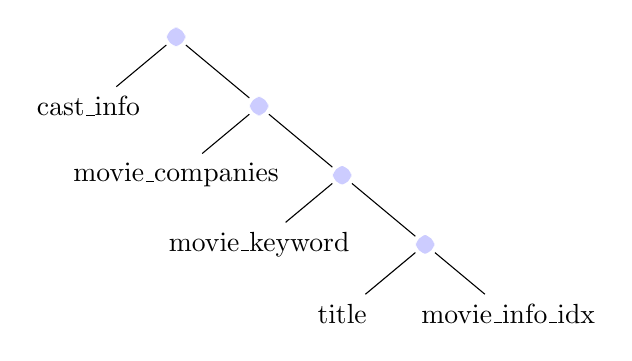
\begin{tikzpicture}[sibling distance=6em, level distance = 2.5em,
  every node/.style = { shape= rectangle, rounded corners,
    draw =none , align=center,
   % top color=white, bottom color=blue!20
   }]]
  \node[fill=blue!20] { \HashJoin } 
      child {
        node { cast\_info }
      }
      child {
        node[fill=blue!20] {\HashJoin }
          child { node{ movie\_companies} }
          child {
              node[fill=blue!20] { \HashJoin }
                child { node {movie\_keyword} }
                child { node[fill=blue!20] {\HashJoin} 
                             child {node {title}}
                             child {node {movie\_info\_idx}}
                      }
        }
    }
  ;
\end{tikzpicture}
 % }
  \label{fig:exp:imdb:postgres}
}\end{subfigure}
%
% cost: 169719.198 ms
% plan: 1298204.64 
% HashJoin(HashJoin(HashJoin(movie_keyword HashJoin(movie_info_idx title)) movie_companies) cast_info)
\begin{subfigure}[\Oracle(time=169.72s, cost=1298.20)]{%
%  \includegraphics[width=0.66\columnwidth,height=2.2cm]{
\scriptsize % \footnotesize
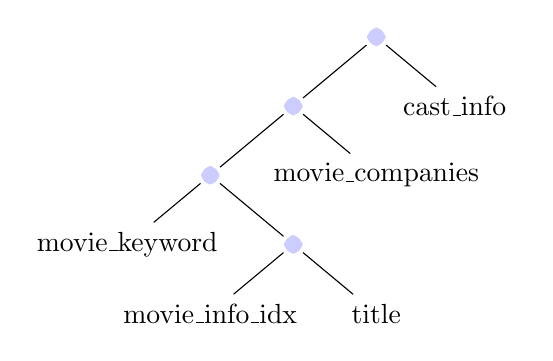
\begin{tikzpicture}[sibling distance=6em, level distance = 2.5em,
  every node/.style = { shape= rectangle, rounded corners,
    draw =none , align=center,
   % top color=white, bottom color=blue!20
   }]]
  \node[fill=blue!20] { \HashJoin } 
      child {
        node[fill=blue!20] {\HashJoin }
          child {
              node[fill=blue!20] { \HashJoin }
                child { node {movie\_keyword} }
                child { node[fill=blue!20] {\HashJoin} 
                             child {node {movie\_info\_idx}}
                             child {node {title}}
                      }
                }
          child { node{ movie\_companies} }
            }
      child {
        node { cast\_info }
      }
      
  ;
\end{tikzpicture}
  \label{fig:exp:imdb:oracle}
}\end{subfigure}
%
\begin{subfigure}[\QIT (time=176.92s, cost=1946.60)]{%
%  \includegraphics[width=0.66\columnwidth,height=2.2cm]{
\scriptsize % \footnotesize
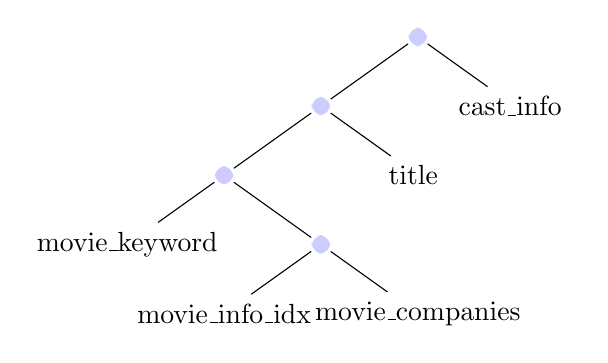
\begin{tikzpicture}[sibling distance=7em, level distance = 2.5em,
  every node/.style = { shape= rectangle, rounded corners,
    draw =none , align=center,
   % top color=white, bottom color=blue!20
   }]]
  \node[fill=blue!20] { \HashJoin } 
      child {
        node[fill=blue!20] {\HashJoin }
          child {
              node[fill=blue!20] { \HashJoin }
                child { node {movie\_keyword} }
                child { node[fill=blue!20] {\HashJoin} 
                             child {node {movie\_info\_idx}}
                             child {node {movie\_companies}}
                      }
                }
          child { node{ title } }
            }
      child {
        node { cast\_info }
      }
  ;
\end{tikzpicture}
%  }
  \label{fig:exp:imdb:qit}
}\end{subfigure}
%
\begin{subfigure}[\QDPO (time=169.43s, cost=2687.73)]{%
%  \includegraphics[width=0.66\columnwidth,height=2.2cm]{
\scriptsize % \footnotesize
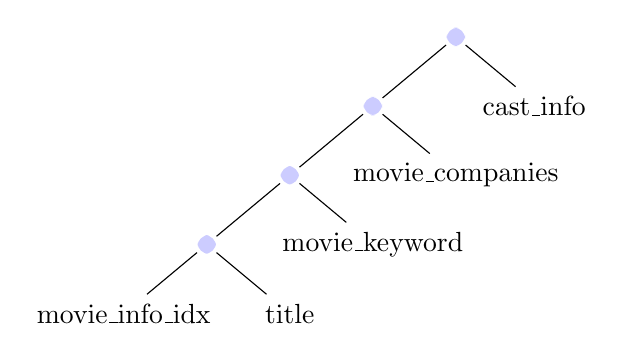
\begin{tikzpicture}[sibling distance=6em, level distance = 2.5em,
  every node/.style = { shape= rectangle, rounded corners,
    draw =none , align=center,
   % top color=white, bottom color=blue!20
   }]]
  \node[fill=blue!20] { \HashJoin } 
      child {
        node[fill=blue!20] {\HashJoin }
          child {
              node[fill=blue!20] { \HashJoin }
                child { node[fill=blue!20] {\HashJoin} 
                             child {node {movie\_info\_idx}}
                             child {node {title}}
                      }
                child { node {movie\_keyword} }
                }
          child { node{ movie\_companies} }
            }
      child {
        node { cast\_info }
      }
      
  ;
\end{tikzpicture}
  \label{fig:exp:imdb:qdpo}
}\end{subfigure}
%
%
\caption{Visualization of plans from \Postgres, \Oracle, \LLMQO (\QIT), \LLMQO (\QDPO) on a query of \imdb}
\label{fig:caststudy:example_imdb}

\end{figure*}

\comment{
\begin{figure*}[t]
\centering
\begin{subfigure}[\Oracle (time=6.9s, cost=744)]{%
 % \includegraphics[width=0.66\columnwidth,height=2.2cm]{
\scriptsize %\footnotesize
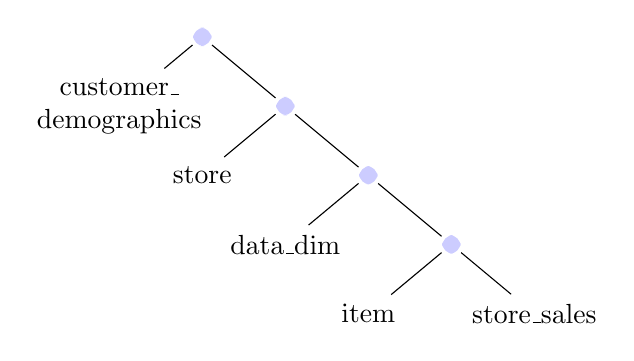
\begin{tikzpicture}[sibling distance=6em, level distance = 2.5em,
  every node/.style = { shape= rectangle, rounded corners,
    draw =none , align=center,
   % top color=white, bottom color=blue!20
   }]]
  \node[fill=blue!20] { \HashJoin } 
      child {
        node {customer\_ \\
        demographics}
      }
      child {
              node[fill=blue!20] { \HashJoin }
                child { node {store} }
                child { node[fill=blue!20] {\HashJoin} 
                             child {node {data\_dim}}
                             child {
              node[fill=blue!20] { \HashJoin }
              {
              child{node {item}}
              child{node {store\_sales}}
              }
                             }
                      }
        }
  ;
\end{tikzpicture}
 % }
  \label{fig:exp:imdb:qdpo}
}\end{subfigure}
%
\begin{subfigure}[\Postgres (Time=3.1s, Cost=518)]{%
%  \includegraphics[width=0.66\columnwidth,height=2.2cm]{
\scriptsize % \footnotesize
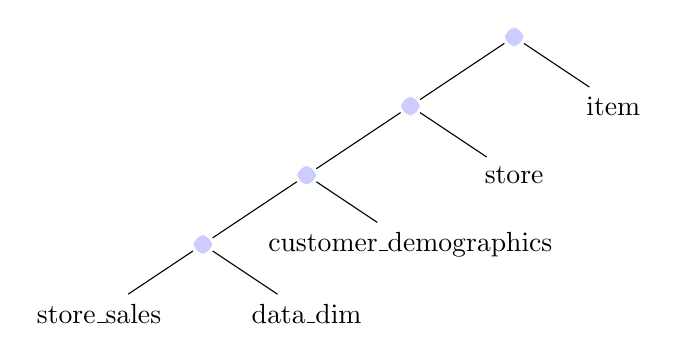
\begin{tikzpicture}[sibling distance=7.5em, level distance = 2.5em,
  every node/.style = { shape= rectangle, rounded corners,
    draw =none , align=center,
   % top color=white, bottom color=blue!20
   }]]
     \node[fill=blue!20] { \HashJoin } 
      child {
        node[fill=blue!20] {\HashJoin }
          child {
              node[fill=blue!20] { \HashJoin }
                child { node[fill=blue!20] {\HashJoin} 
                             child {node {store\_sales}}
                             child {node {data\_dim}}
                      }
                child { node {customer\_demographics} }
                }
          child { node{ store} }
            }
      child {
        node { item }
      }
      ;

\end{tikzpicture}
%  }
  \label{fig:example3:subfigure2}
}\end{subfigure}
%
\begin{subfigure}[\LLMQO(\QIT) \& \LLMQO(\QDPO) (Time=3.3s, Cost=525)]{%
%  \includegraphics[width=0.66\columnwidth,height=2.2cm]{
\scriptsize % \footnotesize
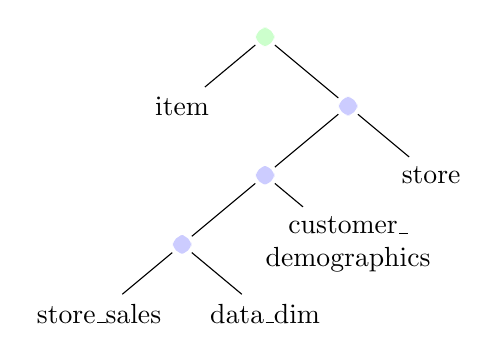
\begin{tikzpicture}[sibling distance=6em, level distance = 2.5em,
  every node/.style = { shape= rectangle, rounded corners,
    draw =none , align=center,
   % top color=white, bottom color=blue!20
   }]]
  \node[fill=green!20] { \NestLoop } 
      child {
        node {item}
            }
      child {
        node[fill=blue!20] {\HashJoin }
          child {
              node[fill=blue!20] { \HashJoin }
                child { node[fill=blue!20] {\HashJoin} 
                             child {node {store\_sales}}
                             child {node {data\_dim}}
                      }
                child { node {customer\_\\
                demographics} }
                }
          child { node{ store} }
      }
  ;
\end{tikzpicture}
  \label{fig:example3:subfigure3}
}\end{subfigure}
\caption{Visualization of plans and planning paths from \Oracle,\Postgres, \LLMQO(\QIT\&\QDPO) on tpl027 of \dsb}
\label{fig:caststudy:example3}
\end{figure*}
}

\comment{
tpl027 45
Oracle 
cost 5616818.46 
Execution Time: 6519.665 ms
HashJoin(customer_demographics HashJoin(store HashJoin(date_dim HashJoin(item store_sales))))

PG 
HashJoin(HashJoin(HashJoin(HashJoin(store_sales date_dim) customer_demographics) store) item)
time 3357.248
time 518168.94 
SFT/DPO
Execution Time: 8799.251 ms
cost 523602.32 
NestLoop(item HashJoin(HashJoin(HashJoin(store_sales date_dim) customer_demographics) store))
LLMQO(DPO)+

HashJoin(item HashJoin(HashJoin(HashJoin(store_sales date_dim) customer_demographics) store))
time 3390.442
cost 518464.11 
}
\comment{
\begin{figure}[t]
\centering
\begin{subfigure}[\Postgres (Time=44s, Cost=298)]{%
 % \includegraphics[width=0.66\columnwidth,height=2.2cm]{
\scriptsize %\footnotesize
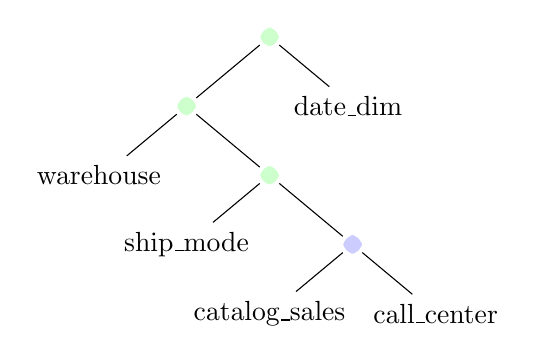
\begin{tikzpicture}[sibling distance=6em, level distance = 2.5em,
  every node/.style = { shape= rectangle, rounded corners,
    draw =none , align=center,
   % top color=white, bottom color=blue!20
   }]]
  \node[fill=green!20] { \NestLoop } 
      child {
        node[fill=green!20] { \NestLoop }
          child { node{ warehouse } }
          child {
              node[fill=green!20] { \NestLoop }
                child { node {ship\_mode} }
                child { node[fill=blue!20] {\HashJoin} 
                             child {node {catalog\_sales}}
                             child {node {call\_center}}
                      }
                }
            }
      child {
        node { date\_dim }
      }
  ;
\end{tikzpicture}
 % }
  \label{fig:example:subfigure1}
}\end{subfigure}
%
\begin{subfigure}[\LLMQO (\QIT\&\QDPO)(Time=2s, Cost=304)]{%
%  \includegraphics[width=0.66\columnwidth,height=2.2cm]{
\scriptsize % \footnotesize
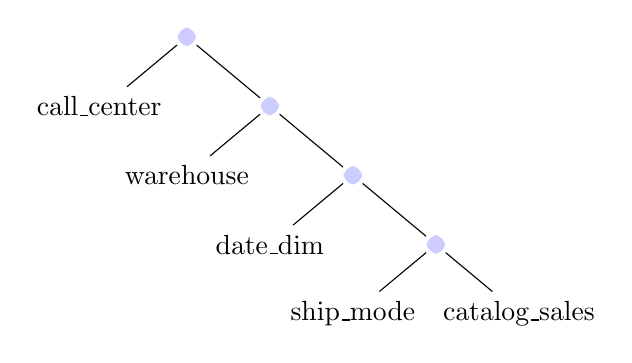
\begin{tikzpicture}[sibling distance=6em, level distance = 2.5em,
  every node/.style = { shape= rectangle, rounded corners,
    draw =none , align=center,
   % top color=white, bottom color=blue!20
   }]]
  \node[fill=blue!20] { \HashJoin } 
      child {
        node { call\_center }
      }
      child {
        node[fill=blue!20] {\HashJoin }
          child { node{ warehouse} }
          child {
              node[fill=blue!20] { \HashJoin }
                child { node {date\_dim} }
                child { node[fill=blue!20] {\HashJoin} 
                             child {node {ship\_mode}}
                             child {node {catalog\_sales}}
                      }
        }
    }
  ;
\end{tikzpicture}
%  }
  \label{fig:example2:subfigure2}
}\end{subfigure}
%
\caption{Visualization of plans and planning paths from \Postgres, \LLMQO (\QIT),\LLMQO (\QDPO) on tpl099 of \dsb.}
\label{fig:caststudy:example2}
\end{figure}
}

%tpl040_88
%PG:
%NestLoop(NestLoop(HashJoin(HashJoin(catalog_sales date_dim) catalog_returns) warehouse) item)
% cost:342559.29 
% time:4494.099 ms

%Oracle: HashJoin(HashJoin(HashJoin(date_dim HashJoin(catalog_returns catalog_sales)) item) warehouse)
% time:2260.605
% cost:368000.69 

%SFT
% NestLoop(NestLoop(NestLoop(catalog_returns HashJoin(catalog_sales date_dim)) warehouse) item)
% time:106079.119
% cost:1218602.04 

%DPO
%HashJoin(HashJoin(HashJoin(catalog_returns HashJoin(catalog_sales date_dim)) item) warehouse)
%time:2184.744
%cost:342311.64
\begin{figure*}[t]
\centering
\begin{subfigure}[\Postgres (time=4.49s, cost=342.56)]{%
 % \includegraphics[width=0.66\columnwidth,height=2.2cm]{
\scriptsize %\footnotesize
% NestLoop(NestLoop(HashJoin(HashJoin(catalog_sales date_dim) catalog_returns) warehouse) item)
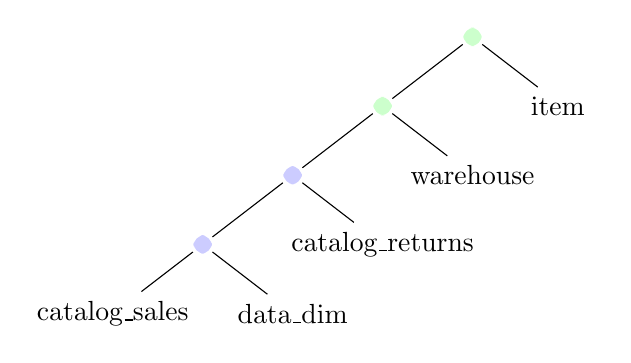
\begin{tikzpicture}[sibling distance=6.5em, level distance = 2.5em,
  every node/.style = { shape= rectangle, rounded corners,
    draw =none , align=center,
   % top color=white, bottom color=blue!20
   }]]
     \node[fill=green!20] { \NestLoop } 
      child {
        node[fill=green!20] {\NestLoop }
          child {
              node[fill=blue!20] { \HashJoin }
                child { node[fill=blue!20] {\HashJoin} 
                             child {node {catalog\_sales}}
                             child {node {data\_dim}}
                      }
                child { node {catalog\_returns} }
                }
          child { node{ warehouse} }
            }
      child {
        node { item }
      }
      ;
\end{tikzpicture}
 % }
  \label{fig:exp:dsb:postgres}
}\end{subfigure}
%
%
%Oracle: HashJoin(HashJoin(HashJoin(date_dim HashJoin(catalog_returns catalog_sales)) item) warehouse)
% time:2260.605
% cost:368000.69 
\begin{subfigure}[\Oracle (time=2.26s, cost=368.00)]{%
%  \includegraphics[width=0.66\columnwidth,height=2.2cm]{
\scriptsize % \footnotesize
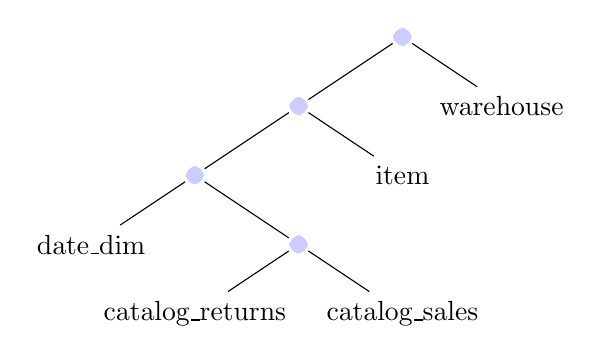
\begin{tikzpicture}[sibling distance=7.5em, level distance = 2.5em,
  every node/.style = { shape= rectangle, rounded corners,
    draw =none , align=center,
   % top color=white, bottom color=blue!20
   }]]
     \node[fill=blue!20] { \HashJoin } 
      child {
        node[fill=blue!20] {\HashJoin }
          child {
              node[fill=blue!20] { \HashJoin }
                child { node {date\_dim} }
                child { node[fill=blue!20] {\HashJoin} 
                             child {node {catalog\_returns}}
                             child {node {catalog\_sales}}
                      }
                }
          child { node{ item} }
            }
      child {
        node { warehouse }
      }
      ;

\end{tikzpicture}
%  }
  \label{fig:exp:dsb:oracle}
}\end{subfigure}
%% NestLoop(NestLoop(NestLoop(catalog_returns HashJoin(catalog_sales date_dim)) warehouse) item)
% time:106079.119
% cost:1218602.04 
\begin{subfigure}[\QIT (time=106.08s, cost=1218.60)]{%
%  \includegraphics[width=0.66\columnwidth,height=2.2cm]{
\scriptsize % \footnotesize
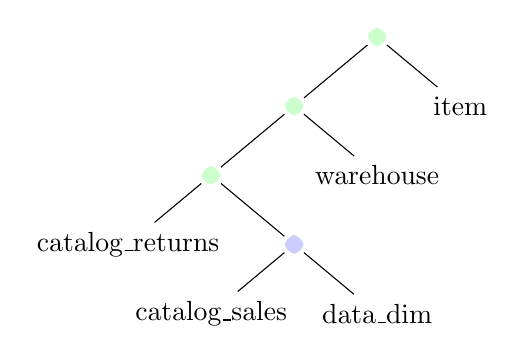
\begin{tikzpicture}[sibling distance=6em, level distance = 2.5em,
  every node/.style = { shape= rectangle, rounded corners,
    draw =none , align=center,
   % top color=white, bottom color=blue!20
   }]]
  \node[fill=green!20] { \NestLoop } 
      child {
        node[fill=green!20] {\NestLoop }
          child {
              node[fill=green!20] { \NestLoop }
                child { node {catalog\_returns} }
                child { node[fill=blue!20] {\HashJoin} 
                             child {node {catalog\_sales}}
                             child {node {data\_dim}}
                      }
                }
          child { node{ warehouse} }
      }
    child {
        node {item}
            }
  ;
\end{tikzpicture}
  \label{fig:exp:dsb:qit}
}\end{subfigure}
%HashJoin(HashJoin(HashJoin(catalog_returns HashJoin(catalog_sales date_dim)) item) warehouse)
%time:2184.744
%cost:342311.64
\begin{subfigure}[\QDPO (time=2.18s, cost=342.31)]{%
%  \includegraphics[width=0.66\columnwidth,height=2.2cm]{
\scriptsize % \footnotesize
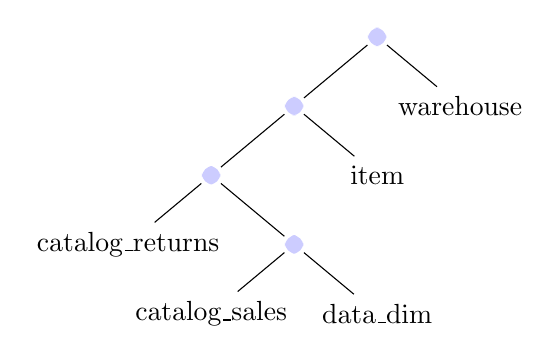
\begin{tikzpicture}[sibling distance=6em, level distance = 2.5em,
  every node/.style = { shape= rectangle, rounded corners,
    draw =none , align=center,
   % top color=white, bottom color=blue!20
   }]]
  \node[fill=blue!20] { \HashJoin } 
    child {
        node[fill=blue!20] {\HashJoin }
          child {
              node[fill=blue!20] { \HashJoin }
                child { node {catalog\_returns} }
                child { node[fill=blue!20] {\HashJoin} 
                             child {node {catalog\_sales}}
                             child {node {data\_dim}}
                      }
                }
          child { node{ item} }
      }
    child {
        node {warehouse}
            }
  ;
\end{tikzpicture}
  \label{fig:exp:dsb:qdpo}
}\end{subfigure}


\caption{Visualization of plans from \Postgres, \Oracle, \LLMQO(\QIT), \LLMQO(\QDPO) on a query of \dsb}
\label{fig:caststudy:example_dsb}
\end{figure*}

We conduct a case study to investigate specific plans generated by \Postgres, \Oracle, and \LLMQO.
In Fig.~\ref{fig:caststudy:example_imdb}, we visualize the plans from a query with 5 tables on \imdb. 
As shown in Fig.~\ref{fig:exp:imdb:postgres}, \Postgres selects the query plan with the lowest estimated cost, even though it spends the longest execution time, indicating a misestimation of the plan cost. In further investigation, we identify that the inaccurate cost estimation arises from an underestimation of cardinality. Specifically, for the topmost hash join in Fig.~\ref{fig:exp:imdb:postgres}, the cardinality of the right sub-plan is underestimated by a factor of 30. Typically, a \HashJoin  builds an in-memory hash table on the smaller input to avoid hash table overflow~\cite{graefe1994sort}. However, the underestimation of cardinality causes \Postgres to build the hash table on the right sub-plan that ultimately turns out to incur a larger join size, resulting in a worse real performance. 
In contrast, as shown in Fig.~\ref{fig:exp:imdb:qit}-\ref{fig:exp:imdb:qdpo}, 
% \LLMQO generates efficient plans for the query by reordering the join operators, and the plan will construct the hash table over a smaller table.
\LLMQO generates efficient plans with different join orders, where the hash join builds the hash table on the smaller input table. 

Fig.~\ref{fig:caststudy:example_dsb} illustrates another query with template tpl040 on \dsb. 
In this case, we observe that the\Oracle's plan is superior to that of \Postgres. 
%就是那个多出来的 nest loop,从0.1 s左右到了 102 s
In addition, we find that \LLMQO(\QIT) generates a plan similar to that of \Postgres, but it takes significantly longer to execute. 
% In Fig.~\ref{fig:exp:dsb:qit}, 
% the '\NestLoop' operator used to join `catalog\_returns' with `\HashJoin(catalog\_sales date\_dim)' consumes 101.8 seconds, dominating the overall execution time of the plan.
% In Fig.~\ref{fig:exp:dsb:qit}, the nested loop join over catalog\_returns and the intermediate result of the join between catalog\_sales and date\_dim consumes 101.8 seconds, dominating the overall execution time of the plan.
In Fig.~\ref{fig:exp:dsb:qit}, the '\NestLoop' operator over catalog\_returns and the intermediate result of the join between catalog\_sales and date\_dim consumes 101.8 seconds, dominating the overall execution time of the plan.
Among the four baselines, \LLMQO (\QDPO) achieves the best performance.
The training of \QDPO enables \LLMQO to learn on the collected preference data from \Oracle and generate a performant plan for the given query, as shown in Fig.~\ref{fig:exp:dsb:qdpo}.
%adjusting the join order between 'item' and 'warehouse', and changing the \NestLoop into \HashJoin.
The comparison between \LLMQO (\QIT) and \LLMQO (\QDPO) confirms that \QIT stage empowers the LLM to generate a valid plan through imitating generic optimizers, and \QDPO stage further guides the the generation of more efficient plans by learning from different optimizers. Our proposed autoregressive generation process fosters new and efficient plans.

\begin{figure}
  \centering
 \includegraphics[width=0.36\textwidth]{figures/inference_efficiency/inference_time-figure0.pdf}
  \caption{The average inference time on three query sets}
\label{fig:exp:inference_efficiency}
    \vspace{-2.5ex}
\end{figure}

\subsection{Plan Generation Time}
\label{sec:exp:time}
To evaluate the efficiency of plan generation for \LLMQO, we assess the average plan generation latency for input queries across three datasets. 
%The output generation is an iterative process where the LLM predicts and appends the token one at a time until it reaches a stopping condition or a specified token limit. 
% vLLM~\cite{kwon2023efficient} is an open-source and community-maintained library known for its efficient memory management and support across a wide range of accelerators. In our experiments, we employ vLLM as the inference framework to enhance the efficiency of the inference stage. 
Fig.~\ref{fig:exp:inference_efficiency} displays the average plan generation latency using LLaMA3-8B on a single A100 or H100 GPU.
%conclusion1 横着看: DSB sequence length更长 所以需要更多时间 相比于IMDB/JOB- light
%conclusion2 纵着看:batch size更大的时候可以很好利用显存资源-> latency更短 fully utilize resources on GPU.
The more complex the query, the longer the expected output response and the corresponding generation time.
%The inference time is observed to be longer as the output sequence length increases.  
Among the three datasets, \dsb exhibits the longest inference time because its queries involve more tables and joins compared to \imdb and \job.
In general, we observe that latency decreases as batch size increases due to more efficient utilization of computational and memory resources provided by the hardware.
For \dsb on A100, the inference latency does not decrease when the batch size increases from 32 to 64, as a batch size of 32 is sufficient to exploit GPU resources, given the complicated queries in \dsb.
In summary, complicated queries on large database instances can enjoy more benefits from \LLMQO. Ongoing techniques for speeding up LLM inference, such as KV cache, continuous batching and speculative decoding~\cite{DBLP:conf/icml/LeviathanKM23} will improve the utility of \LLMQO.
%It is worth noting that the latency in \LLMQO
%is justifiable given that the combined inference time and execution time is lower than that of baseline methods, especially for the most complicated \dsb queries. This indicates that the complex queries benefit more from our method.







